%%%%%%%%%%%%%%%%%%%%%%%%%%%%%%%%%%%%%%%%%
% Beamer Presentation
% LaTeX Template
% Version 1.0 (10/11/12)
%
% This template has been downloaded from:
% http://www.LaTeXTemplates.com
%
% License:
% CC BY-NC-SA 3.0 (http://creativecommons.org/licenses/by-nc-sa/3.0/)
%
%%%%%%%%%%%%%%%%%%%%%%%%%%%%%%%%%%%%%%%%%

%----------------------------------------------------------------------------------------
%	PACKAGES AND THEMES
%----------------------------------------------------------------------------------------

\documentclass{beamer}
\usepackage{amsmath,amsthm,amssymb,amsfonts,graphicx} % The standard ams packages used very commonly
\usepackage{hyperref} % Used to make links or other things like that relating to the internet.
\usepackage[backend=bibtex, style=numeric]{biblatex}
% \usepackage{xfrac} % Provides a pretty way to write fractions inline. Use \sfrac{}{}
% \usepackage{dsfont} % This gives the neat font \mathbb{} which is comparable in style to \mathbb{}
% \usepackage{mathrsfs} % Provides a nice curly font. Use \mathscr{}.
% \usepackage{inputenc, fontenc}
\addbibresource{refs.bib}

%%%%%%%%%%%%%%%%%%%%%%%%%%%%%%%% Operators
%These may be useful and maybe you will want to make more that you think are convenient

\DeclareMathOperator{\Mat}{Mat}
\DeclareMathOperator{\End}{End}
\DeclareMathOperator{\Hom}{Hom}
\DeclareMathOperator{\id}{id}
\DeclareMathOperator{\image}{im}
\DeclareMathOperator{\Imag}{Imag}
\DeclareMathOperator{\rank}{rank}
\DeclareMathOperator{\nullity}{nullity}
\DeclareMathOperator{\trace}{tr}
\DeclareMathOperator{\Spec}{Spec}
\DeclareMathOperator{\Sym}{Sym}
\DeclareMathOperator{\pf}{pf}
\DeclareMathOperator{\Ortho}{O}
\DeclareMathOperator{\rad}{rad}

% Shortcuts for common symbols:
\DeclareMathOperator{\C}{\mathbb{C}}
\DeclareMathOperator{\R}{\mathbb{R}}
\DeclareMathOperator{\Q}{\mathbb{Q}}
\DeclareMathOperator{\Z}{\mathbb{Z}}
\DeclareMathOperator{\N}{\mathbb{N}}
\DeclareMathOperator{\F}{\mathbb{F}}
\newtheorem{remark}{Remark}

\newcommand{\p}[1]{\left(#1\right)}
\newcommand{\norm}[1]{\left\lVert#1\right\rVert} % Encircles the argument in || ||. 

\mode<presentation> {

% The Beamer class comes with a number of default slide themes
% which change the colors and layouts of slides. Below this is a list
% of all the themes, uncomment each in turn to see what they look like.

%\usetheme{default}
%\usetheme{AnnArbor}
%\usetheme{Antibes}
%\usetheme{Bergen}
%\usetheme{Berkeley}
%\usetheme{Berlin}
%\usetheme{Boadilla}
%\usetheme{CambridgeUS}
%\usetheme{Copenhagen}
%\usetheme{Darmstadt}
%\usetheme{Dresden}
%\usetheme{Frankfurt}
%\usetheme{Goettingen}
%\usetheme{Hannover}
%\usetheme{Ilmenau}
%\usetheme{JuanLesPins}
%\usetheme{Luebeck}
\usetheme{Madrid}
%\usetheme{Malmoe}
%\usetheme{Marburg}
%\usetheme{Montpellier}
%\usetheme{PaloAlto}
%\usetheme{Pittsburgh}
%\usetheme{Rochester}
%\usetheme{Singapore}
%\usetheme{Szeged}
%\usetheme{Warsaw}

% As well as themes, the Beamer class has a number of color themes
% for any slide theme. Uncomment each of these in turn to see how it
% changes the colors of your current slide theme.

%\usecolortheme{albatross}
%\usecolortheme{beaver}
%\usecolortheme{beetle}
%\usecolortheme{crane}
%\usecolortheme{dolphin}
%\usecolortheme{dove}
%\usecolortheme{fly}
%\usecolortheme{lily}
%\usecolortheme{orchid}
%\usecolortheme{rose}
%\usecolortheme{seagull}
%\usecolortheme{seahorse}
%\usecolortheme{whale}
%\usecolortheme{wolverine}

%\setbeamertemplate{footline} % To remove the footer line in all slides uncomment this line
%\setbeamertemplate{footline}[page number] % To replace the footer line in all slides with a simple slide count uncomment this line

%\setbeamertemplate{navigation symbols}{} % To remove the navigation symbols from the bottom of all slides uncomment this line
}


%----------------------------------------------------------------------------------------
%	TITLE PAGE
%----------------------------------------------------------------------------------------

\title[Dynamical organization of brain using TDA]{Towards a new approach to reveal dynamical
organization of the brain using topological data analysis} % The short title appears at the bottom of every slide, the full title is only on the title page

\author{Jay Patel} % Your name
\institute[OSU] % Your institution as it will appear on the bottom of every slide, may be shorthand to save space
{
The Ohio State University \\ % Your institution for the title page
\medskip
\textit{patel.3316@osu.edu} % Your email address
}
\date{\today} % Date, can be changed to a custom date

\begin{document}

\begin{frame}
    \titlepage % Print the title page as the first slide
\end{frame}

\begin{frame}{Premise}
    \begin{itemize}
        \item Little is known about how the brain adapts in order to efficiently complete one task vesus another \pause
        \item Most previous work focuses on analyzing co-fluctuations of the brain at different times \pause
        \item Collapsing the data into co-fluctuations will make us lose useful information about the overall dynamical organization \pause
        \item This paper takes the existing data and ananlyzes it at the ``single participant level" \pause
        \item The approach of this paper is able ot probe within and between task transitions of about ($~$4-9 seconds) \pause
        \item They observe that the revealed individual differences in the dynamical organization of the subject were predictors of the task performace
    \end{itemize}
\end{frame}

\begin{frame}{Data}
    \begin{itemize}
        \item They used multiple fMRI datasets which are scans of individuals over $~$25  minutes while doing a variaty of tasks \pause
        \item Previously, this data has typically been used in models after some kind of ``averaging'' procedure \pause
        % methods based on sliding-window, single-volume co-activation patterns, wavelets, change-point detection, deconvolution, multiplication of temporal derivatives, and temporal Independent Component Analysis have been proposed
        \item The previous approaches have been unable to reveal the optimal temporal and spatial scales which best probe clinically and behearviorly relevant brain dynamics \pause
        \item Additionally, they are unable to determine if the brain dynamics are best thought of as continuous or discrete or able to tell whether a particular brain activity is healthy or not
    \end{itemize}
\end{frame}

\begin{frame}{Pipeline}
    \begin{figure}
        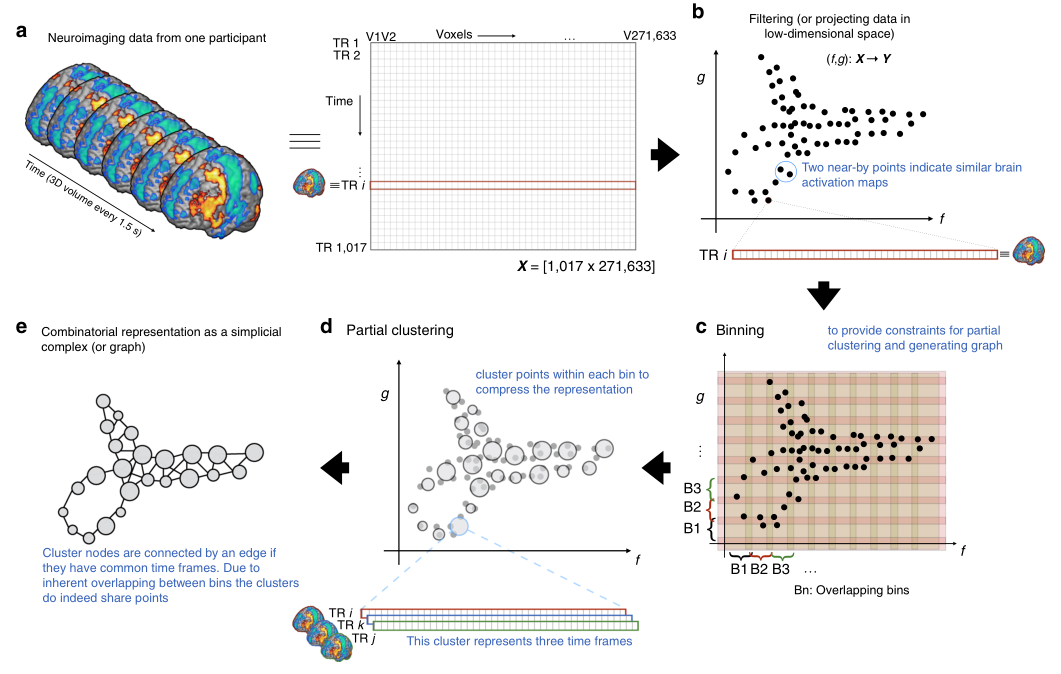
\includegraphics[width = 0.8\linewidth]{fig1.png}
        \caption{The method used to convert the 4-dimensional fMRI data into a simplicial complex. Steps b-e are a part of Mapper (the TDA-based algorithm/tool the authors used).}
    \end{figure}
\end{frame}

\begin{frame}{How Mapper works}
    \begin{itemize}
        \item Step b the filtering into $\R^2$ is done using something called Stochastic Neightborhood Estimation. \pause SNE, is used over traditional methods like PCA because SNE allows us to preserve the local structure of the origional data \pause
        \item Step c is just binning the space using the provided parameters: number of bins and the percentage overlap between bins\pause
        \item Step d goes through each bin, and performs single-linkage clustering in order to form clusters of nearby points\pause 
        \item Step e treats each cluster as a vertex of a graph and adds an edge between two vertices if they shared a point \cite{mapper}
        % The authors used something called the CMP dataset which is pretty standard and after applying mapper to each participant in CMP, they want to analyze the properties of each person's graph
    \end{itemize}
\end{frame}



\begin{frame}[allowframebreaks]
\frametitle{References}
\printbibliography
\end{frame}

% %------------------------------------------------

\begin{frame}
\Huge{\centerline{The End}}
\end{frame}

%----------------------------------------------------------------------------------------

\end{document} 